India has a slow judiciary --- courts are clogged with large backlogs \autocite{moog1992delays, debroy2008justice, dutta2019modernise}. As of 8th December 2021, over forty-one million cases were pending across district courts \autocite{njdg2021}. Slow judiciaries have adverse consequences on the structure and efficiency of markets and the quality of life of citizens \autocite{world2004world, chemin2007impact, rao2020institutional}. Therefore, minimising unnecessary judicial delays could help improve enforcement and enhance the overall rule of law. It is estimated that judicial delays cost India around 1.5\% of its GDP annually.\footcite{dey2016_cost} Against this backdrop, it is hardly surprising that tackling judicial delay has increasingly become a top priority for Indian judges and policymakers.

Link number of cases to State GDP. No of cases is directly linked to the economic activity. If delay hinders performance, then it will hurt the well performing states more. State GDP will suffer and it will have asymmetrical impact on Indian GDP. Insert the figure of SGDP and no of NI 138 cases.

One reason for the large burden on courts is believed to be the large share of \gls{ni} cases.\footnote{In particular, \S~138 of the Negotiable Instruments Act (Dishonour of cheque for insufficiency, etc., of funds in the account). Act 26 of 1881} As per the \gls{lci}, they represent 6.5\% and 7.8\% of all institutions and pendency in Indian courts, respectively \autocite{lci2014_arrears}. As per one order of the Supreme Court of India, they reflect more than 15\% of all criminal cases in the District Courts \autocite{sc2020_makwanavstate}. As per another order, they constitute 30\% of the total pendency in courts.\footcite[Similarly, a study published by the Department of Justice briefly touches on the burden of such cases on the judiciary and posits that they constitute 34\% of pending criminal cases in Maharashtra.][]{sc2020_138, mahadik2018_maharashtra}

Such knowledge is based on the assumption that cheque dishonour cases are a large burden on the judiciary and has thus focused on expediting disposal. For example, \gls{lci} (2008), by relying on newspaper reports concerning the proportion of cheque dishonour cases, recommended setting up Fast Track Magisterial Courts \autocite{lci2008_138, bhan2015_placing}. However, it did not define \textit{fast-track courts} or give guidance concerning how and where they would operate. Developing this work, \textcite{sridhar2017_cheque} examined the behaviour of cheque dishonour cases in the Indian courts by looking at over 67000 cases. In most cases, it found that resolution is delayed well beyond statutorily prescribed timelines and that certain banks and financial institutions are frequent complainants \autocite{sridhar2017_cheque}. As per our own estimates, less than 20\% of the cases get disposed within the stipulated timeline (see Figure \ref{fig:stateSurvival} for comparison across states in India).

\begin{figure}[h]
 \centering
 \caption{Survival probability of cases across States}\label{fig:stateSurvival}
 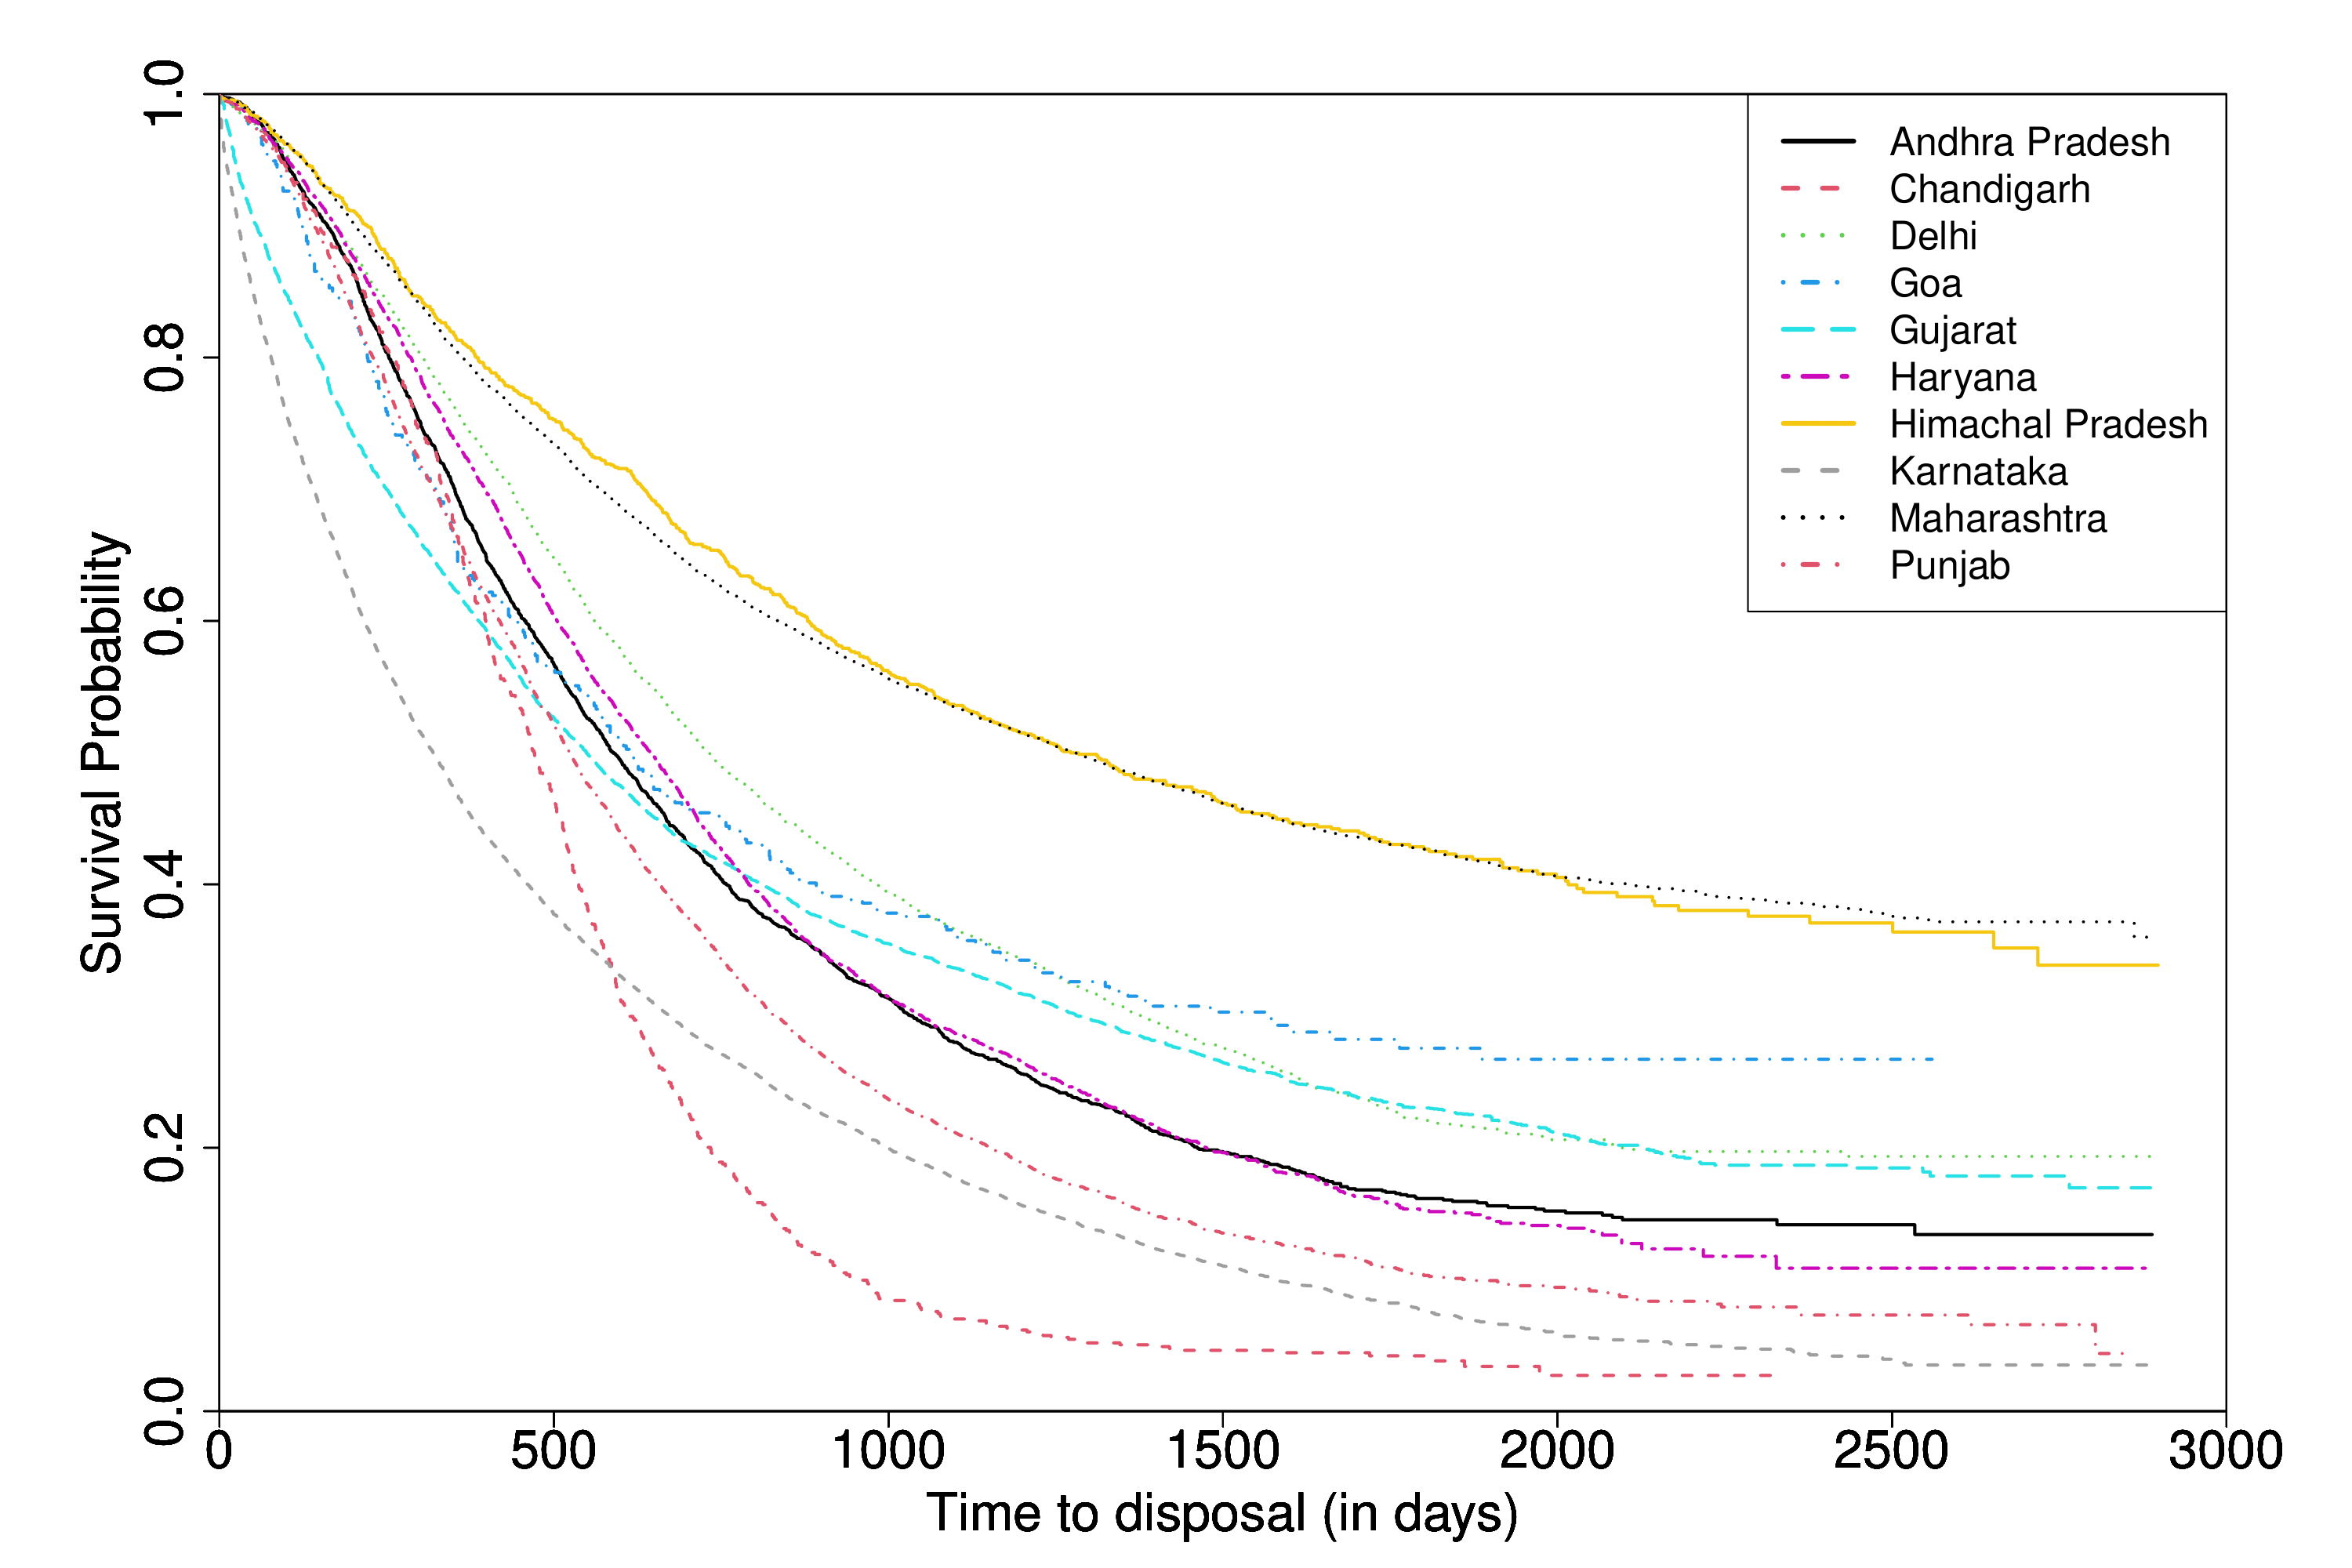
\includegraphics[width = 0.9\textwidth]{surv_states-1.png}
\end{figure}

To this end, in 2020, the Supreme Court of India took on board a suo-motu case concerning the “expeditious trial of cases under section 138 of the Negotiable Instruments Act 1881” \autocite{sc2020_138}. Among other directions, the court (i) appointed a \gls{coe}\footnote{Headed by Hon’ble Mr Justice RC Chavan, former Judge of the Bombay High Court.} and (ii) appointed Amici Curiae to assist the court,\footnote{Mr Sidharth Luthra (Sr Advocate) and Mr K Parameshwar (Advocate).} to study processes to expedite disposal of complaints under \S~138 of the \gls{ni}. This is in a series of interventions targeted to understand cheque dishonour cases in India. As \cref{sec:history} shows, most knowledge and development concerning such cases in India has come from government institutions, i.e. the \gls{lci} and the judiciary. The Amici appointed by the Supreme Court also made recommendations to expedite the disposal of cases. This included (i) increasing the use of pre- and post-summons mediation, (ii) expediting the service of summons to reduce absconsion, (iii) addressing the multiplicity of proceedings, etc.\footcite[For details see ]{amicus2020_submission} 

This study, based on orders of the Supreme Court and the report of the Amici Curiae, attempts to assess the effect of suggested interventions on the expeditious trial of cases under \S~138 of the \gls{ni}. First, we estimate the volume of NI 138 cases in the subordinate courts. Given the disagreement, any acceptance among policymakers that \gls{ni} cases (\textit{cheque dishonour cases} hereinafter) are the reason for India's slow judiciary is likely to lead to misguided solutions. The misrepresentation could lead to diverting resources from other routes of judicial reform. Thus, one requires a more detailed analysis of the proportion of such cases, their causes, timelines, etc. This information can help judges and policymakers better target interventions.\footcite[For the importance of accurate judicial data, see][]{damle2020_ecourtsData, daksh2020_data, damle2020_land}

Second, we estimate the likely impact of some select recommendations of the Amici Curiae and the Supreme Court. This can help the court gauge how effective their recommended reforms are likely to be. As we show, some of the recommendations can end up being counterproductive. We, thus, also demonstrate the need for judicial decision-making to be rooted in data.

The rest of this paper is organised as follows: after this introduction, \cref{sec:history} elaborates the history of cheque dishonour provisions in India and their relation with judicial delays. In \cref{sec:select-case-char}, based on the recommendations of the Amici Curiae and the Supreme Court, we figure out the key case characteristics that can be targeted by direct court interventions. \Cref{sec:methodology} describes the methodology, and \cref{sec:results} presents the results thereof. Finally, \cref{sec:conclusion} concludes the paper and presents the way forward.

\section{Cheque dishonour and judicial delays} \label{sec:history}

The \acrlong{ni} was enacted to define the law relating to promissory notes, bills of exchange, and cheques (for an explanation of \S~138, see Appendix \ref{app:understanding}).\footcite{ind1881_niAct} To increase the culture regarding the use of cheques and enhance the credibility of the instrument, the Act was amended in 1988.\footcite{niAmend1988} A new chapter (\S\S~138 to 142) was incorporated for penalties in the event of dishonour of cheques due to insufficient funds in the account of the drawer of the cheque. However, it aimed to include adequate safeguards to prevent harassment of honest drawers. \S~138 provided for the circumstances under a drawer can be penalised for the dishonour of a cheque.

However, by 2001, these provisions were thought not to have had the desired effect.\footcite{stdcomm2001_138niAct} While the punishment was thought to be inadequate, courts could not dispose of cases in a time-bound manner due to the large number of cases pending across the country. Given the large burden on courts, a Working Group was constituted the same year to review \S~138 of the \gls{ni} and make recommendations regarding the changes needed to effectively achieve the purpose of the section.\footcite{wg2001_138} In light of the recommendations of the Working Group, the government decided to bring further amendments to the Act. Among others, the amendments included:

\begin{enumerate}[label=(\alph*)]
 \item increasing the punishment from one year to two years;
 \item providing discretion to the court to waive the period of one month for taking cognisance of a case;
 \item prescribing the procedure for dispensing with preliminary evidence of the complainant;
 \item prescribing the procedure for service of summons via speed post or impanelled private couriers;
 \item providing for summary trials; and
 \item making the offence compoundable.
\end{enumerate}

The amendments aimed at speedy disposal of cheque dishonour cases through their summary trial and making the cases compoundable. The punishment provided under \S~138 also was enhanced from one year to two years. These legislative
reforms aimed to encourage the usage of cheques so that regular business transactions and settlement of liabilities could be ensured. The amendments were considered by the Lok Sabha Standing Committee on Finance, which recommended that given the large burden on courts, the proposed amendments be coupled with the creation of specialised courts for \S~138 cases.\footcite{stdcomm2001_138niAct} However, the subsequent Amending Act did not reference specialised courts.\footcite{niAmend2002} 

\gls{lci} took up the proposal for specialised courts in 2008. According to the Commission, the credibility of the financial sector was facing setbacks due to the large pendency of dishonoured cheque cases. Relying on an array of judgments by the Supreme Court of India concerning speedy trials,\footcite{sc1978_khatoon, sc1981_champalal, sc2005_surinder, sc2008_krishna} the Commission recommended the introduction of fast track courts to address cases concerning dishonour of cheques under \S~138 of the Act. However, it did not comment on the number or expected workload of such courts.\footcite{lci2008_138} The need for additional courts was re-iterated by \gls{lci} in 2009.\footcite{lci2009_reforms}

While \gls{lci} has focused on the need for more courts, the Supreme Court has provided assistance in implementing the amendments. In 2014, noting that the prime reason for the delays in \S~138 case is the absence of the accused, the Court held that the magistrate should adopt a pragmatic and realistic approach such as issuing notices and summons via e-mail or push notification to ensure delivery.\footcite{sc2014_iba} In 2018, the court directed banks to give the details of the e-mail of the accused to the complainant for service through e-mail. The court also directed that: (i) cases must be dealt with summarily, (ii) the evidence of the complainant must be conducted within three months, (iii) an endeavour must be made to conclude the trial within six months, (iv) the trial, as far as practicable, must be held on a day-to-day basis, and (v) High Courts may pass additional localised directions for speedy disposal of cases.\footcite{sc2018_meters}

The Act was also amended in 2015 and 2018 to - clarify the appropriate area of jurisdiction where cheque dishonour cases can be filed,\footcite{niAmend2015} and grant power to courts to grant interim compensation, respectively.\footcite{niAmend2018} In particular, the \citetitle{niAmend2015} 2015 aimed to address the difficulties faced by the payee or lender in filing cases under \S~138 due to a lack of clarity concerning the appropriate forum. It thus inserted specific provisions concerning the jurisdiction for an offence under \S~138, hoping to ensure that a fair trial of cases under \S~138 is conducted keeping in view the parties' interests by clarifying the territorial jurisdiction for trying cases.

On the other hand, the \citetitle{niAmend2018} 2018 aimed to address the delays caused by unscrupulous drawers of dishonoured cheques due to easy filing of appeals and obtaining stay on proceedings. As a result, the payee would have to spend considerable time and resources in court proceedings to realise the value of the cheque. To discourage frivolous and unnecessary litigation, it inserted a new section to provide that a court trying an offence under section 138 may order the drawer of the cheque to pay interim compensation to the complainant, in a summary trial or a summons case, where he pleads not guilty to the accusation made in the complaint; and in any other case, upon framing of charge.

Lastly, in March 2020, the Supreme Court of India took on board a suo-motu case concerning the “expeditious trial of cases under section 138 of the Negotiable Instruments Act 1881”.\footcite{sc2020_138} As mentioned, the court-appointed Amici Curiae to assist in the matter, which presented its preliminary report to the court in October of the same year. The Amici made several suggestions to expedite trial, which among others, includes:

\begin{enumerate}[label=(\alph*)]
 \item Address jurisdictional issues;
 \item Address multiplicity of proceedings; and
 \item Expedite service of summons to reduce absconsion;
 \item Explore setting up specialised courts;
 \item Increase the use of pre- and post-summons mediation;
 \item Mandate presenting of a plausible defence before conversion from summary to summons trial; and
 \item Summon witnesses only when the accused presents a defence.\footcite{amicus2020_submission}
\end{enumerate}

Noticeably, the recommendations of the Amici Curiae were in line with previously accepted reasons for delays in disposal. While considering the recommendations, the Supreme Court recommended the Government and High Courts take necessary action where possible and held that they should be the subject matter of deliberation by the \gls{coe} appointed in the same case.\footnote{Headed by Hon’ble Mr Justice RC Chavan, former Judge of the Bombay High Court.}

\section{Conceptual framework and hypotheses}
\label{sec:select-case-char}

The recommendations of the Amici Curiae and the Supreme Court target several aspects of a \gls{ni} case. They posit that these aspects likely lead to delays. This study examines six areas that are the targets of these interventions, viz. ---

\begin{enumerate}
\item non-appearance by the accused;
\item trials being run as summons trials;
\item reference to mediation;
\item jurisdictional issues;
\item multiplicity of proceedings;
\item setting up additional \gls{ni} courts.
\end{enumerate}

The case characteristics whose impact we have chosen to examine were determined based on two factors: (1) the importance of that characteristic and (2) the feasibility of finding reliable information about it in the eCourts data. Accordingly, we chose to examine the effect of six case characteristics that map onto the six intervention targets mentioned above. The characteristics we chose are as follows:
\begin{enumerate}
\item The accused fails to appear before the court for at least one hearing;
\item The case is converted to a summons trial;
\item The case is referred to mediation;
\item The case has jurisdictional issues and is transferred to another court, as a result;
\item The case contains a multiplicity of proceedings --- either the dishonoured cheque was issued to satisfy multiple transactions, or multiple cheques were dishonoured;
\item The case was contested.
\end{enumerate}

We discuss the salience of each case characteristic and the accompanying hypotheses below.

\subsection{Non-appearance of the accused} 
\label{sec:non-appe-accus}

\textcite{ostrom2000efficiency}, in a study of nine state criminal trial courts in the United States, find that criminal cases where the defendant absconds take 40--90 days longer to dispose than those where the defendant appears in court.\footnote{The authors attribute this to the fact that in such cases, a separate procedure has to be conducted for the judge to issue a bench warrant to produce the accused before the court.} The defendant failing to appear in court is one of the leading causes for failed hearings. Consequently, delays in case disposal in the United Kingdom \autocite{crownProsecutionService2006_magistrateCourtEfficiency}. Similarly, \textcite{llangasinghe1988_fijiJudicialDelays} found that the accused absconding is the most common reason for delays in case disposal in magistrates' courts in Fiji. The Amici Curiae and the Supreme Court's recommendations are premised on the notion that non-appearance of the accused leads to delays. We, therefore, seek to examine whether this holds good for cheque dishonour cases in India. We test the following hypotheses:

\begin{description}
\item[H$_{1a}$]: cases, where the accused does not appear for one or more hearings, require more days to dispose
\item[H$_{1b}$]: cases, where the accused does not appear for one or more hearings, require more hearings to dispose
\end{description}

\subsection{Conversion to summons trial}
\label{sec:conv-summ-trial}

We could not find empirical studies on the effectiveness of summary trials in reducing case duration. Procedural law governing summary trials in the United States and United Kingdom are premised on the assumption that summary trials would reduce time delays in case disposal \autocite{miller2003}. At the same time, \textcite{miller2003} argues that regardless of the time-savings that may (or may not) result from summary trials, the discretion it gives to courts violates the principle of the right to a trial by jury. Therefore, bearing in mind the Supreme Court and Amici Curiae's recommendation that, to the extent possible, cases should be conducted as summary trials, and they should be converted to summons trials only in specific situations we test the following hypotheses:

\begin{description}
\item[H$_{2a}$]: cases converted to summons trials require more days to dispose
\item[H$_{2b}$]: cases converted to summons trials require more hearings to dispose
\end{description}

\subsection{Cases referred to mediation by the court} \label{sec:furth-exam-cases}

\textcite{buscaglia1997_latinAmericaCourtDelays} find that, in Latin American courts, when judges mandate mediation, it reduces the overall time required to dispose a case.\footnote{They conjecture is that the efficiency gains would result in judges having to dedicate less time to adjudicate such cases.} However, a review of empirical research on the time and cost-effectiveness of court-annexed Alternative Dispute Resolution (ADR), including mediation, by \textcite{wissler2004effectiveness} finds no conclusive relationship between the time required to dispose cases via ADR as compared to going to trial. Some studies reviewed by \textcite{wissler2004effectiveness} find that mediation can increase the duration. Some find that it can decrease the duration, while some find no effect. \textcite{heise2010adr} further finds that participation in ADR does not significantly affect case disposal time. However, cases where the parties choose to settle take less time than ADR. Given the mixed findings on the effect of mediation and the Supreme Court and Amici Curiae's opinion that court-annexed mediation can reduce time to dispose cases, we test the following hypotheses:

\begin{description}
\item[H$_{3a}$]: cases referred to mediation require more days to dispose
\item[H$_{3b}$]: cases referred to mediation require more hearings to dispose
\end{description}

\subsection{Jurisdictional issues}

Prima facie, there are four territorial areas involved in a cheque dishonour case - (i) where the issuer ordinarily resides, (ii) where the payee ordinarily resides, (iii) where the cheque was issued, and (iv) where the cheque was presented. 

Prior to 2015, the \gls{ni} only specified circumstances under which complaints concerning cheque dishonour could be filed. It did not specify the territorial jurisdiction of the courts where such a complaint had to be filed. This resulted in individuals filing cases in locations not readily accessible to the opposite party. Thus, cases would have to be transferred to suitable courts for hearing. In 2015, the Act was amended to provide that complaints can only be filed in a court in whose jurisdiction the bank branch of the payee lies.\footcite{niAmend2015} While this addressed the lack of clarity in the court where complaints had to be filed, invariably, cases commenced in territorial jurisdiction where the accused did not ordinarily reside.\footcite{amicus2020_submission}

Such jurisdictional issues, where cases have to be transferred from one court to another, may lead to delays.\footcite{sc2020_138, amicus2020_submission} We thus test the following hypotheses:

\begin{description}
\item[H$_{4a}$]: Cases with jurisdictional issues require more days to dispose
\item[H$_{4b}$]: Cases with jurisdictional issues require more hearings to dispose
\end{description}

\subsection{Multiplicity of proceedings}

\S~219 of the \gls{crpc} provides that when a person is accused of more than one offence of the same kind committed within twelve months, all offences may be tried together, subject to a maximum of three such offences. Similarly, as per \S~220, if a person commits more than one offence in one transaction, she may be charged with all offences and tried at one trial. Experience has shown that a single financial transaction may lead to the dishonour of multiple cheques. However, under the \gls{crpc}, only three offences and, therefore, the dishonour of only three cheques can be tried together. This has resulted in multiple proceedings involving either the same issuer (accused) or the same transaction. Reducing such multiplicity may reduce the burden on courts. We thus test the following hypotheses:

\begin{description}
\item[H$_{5a}$]: Cases involving a multiplicity of proceedings require more days to dispose
\item[H$_{5b}$]: Cases involving a multiplicity of proceedings require more hearings to dispose
\end{description}

\subsection{Contested cases}
\label{sec:contested_cases_meth}
When cases are contested, parties lead evidence before a court and rebut arguments. This is likely to lead to longer proceedings since courts have to come to reasoned decisions based on the proceedings. On the other hand, uncontested cases use minimal court resources, since parties reach a mutually acceptable decision verified by the court. \textcite{ostrom2000efficiency} find that cases that went to trial took 53--158 days longer to dispose than cases where the defendant pleaded guilty.\footnote{The variation in the average delay is between the different jurisdictions studied.} \textcite{buscaglia1997_latinAmericaCourtDelays}, in a study of judicial efficiency in Latin American courts, find that willingness to litigate increases the duration of court cases and results in a greater backlog of cases. \textcite{crownProsecutionService2006_magistrateCourtEfficiency} finds that, in magistrate courts in the United Kingdom, contested cases typically take a greater number of hearings to dispose than uncontested cases. Contested cases take longer to dispose than uncontested cases. The difference between the time it takes the courts to dispose of uncontested cases compared to contested cases can yield insights into how efficient the court is at handling cases that go to trial, compared to cases where the defendant is willing to settle or compound. We thus test the following hypotheses:

\begin{description}
\item[H$_{6a}$]: Contested cases require more days to dispose
\item[H$_{6b}$]: Contested cases require more hearings to dispose
\end{description}

In summary, these characteristics represent six different events that can take place in the course of litigating the case.\footnote{These are not mutually exclusive. One or more of these events can occur in the same case.} We test whether the event's occurrence affects the case duration and the number of hearings required to dispose it. Table \ref{tab:expected} presents a summary of the expected effects of the identified case characteristics. The potential effectiveness of the Supreme Court and Amici Curiae's recommendation of setting up more \gls{ni} courts can be indirectly tested through this characteristic. 

\begin{longtable}{@{}lcc@{}}
\caption{Expected effects of case characteristics}
\label{tab:expected}\\
\toprule
\multicolumn{1}{c}{\multirow{2}{*}{\textbf{Case characteristic}}} & \multicolumn{2}{c}{\textbf{Expected effect}} \\ \cmidrule(l){2-3} 
\multicolumn{1}{c}{} & \textbf{Duration} & \textbf{Hearings} \\ \midrule
Non-appearance of the accused & + & + \\
Conversion to summons trial & + & + \\
Mediation & - & - \\
Jurisdictional issues & + & + \\
Multiplicity of proceedings & + & + \\
Contested cases & + & + \\ \bottomrule
\end{longtable}

%%% Local Variables:
%%% mode: latex
%%% TeX-master: "paper_chequeDishonour"
%%% End:
